\documentclass{article}
\usepackage[utf8]{inputenc}
\usepackage{tikz}
\usepackage{float}
\usetikzlibrary{shapes,arrows,positioning}

\tikzset{
        block/.style = {draw, fill=white!20, rectangle, minimum height=3em, minimum width=6em},
        sum/.style = {draw, fill=white!20, circle, node distance=1cm},
        input/.style = {coordinate},
        output/.style = {coordinate},
        pinstyle/.style = {pin edge={to-,t,black}},
        ylabel/.style={rotate=90},
    }

\title{ICSI412 Assignment 5: Documentation}
\author{Huang Kaisheng (2020215138@stu.cqupt.edu.cn)}
\date{May. 16th, 2023}

\begin{document}

\maketitle
\newpage

\tableofcontents
\newpage


\section{System Documentation}
This section contains a high-level data flow diagram, list of routines and brief descriptions and some implementation details.
\subsection{High-level Data Flow Diagram}
Figure 1 shows the high level data flow diagram.
\begin{figure}[H]
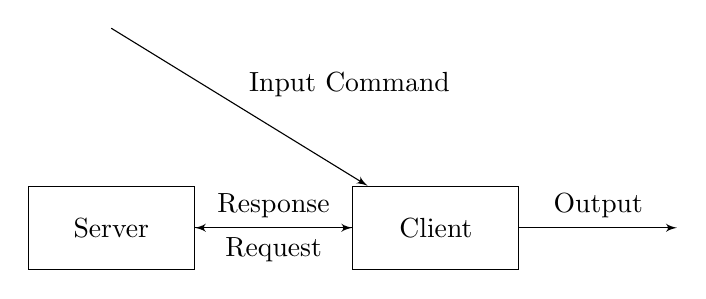
\begin{tikzpicture}[auto, node distance=2cm,>=latex']
    \node [input, name=input] {};
    \node [block, below=of input] (server) {Server};
    \node [block, right=of server] (client) {Client};
    \node [output, right=of client](output) {};

    \draw [->] (input) -- node {Input Command} (client);
    \draw [->] (server) -- node {Response} (client);
    \draw [->] (client) -- node {Request} (server);
    \draw [->] (client) -- node {Output} (output);

\end{tikzpicture}
\caption{Data Flow Diagram}
\end{figure}

\subsection{List of Routines and Brief Descriptions}
\begin{table}[h]
\centering
\begin{tabular}{|p{4cm}|p{9cm}|}
\hline
\textbf{Function} & \textbf{Description} \\ \hline
\texttt{error(const char* msg)} & Displays an error message and terminates the program. \\ \hline
\texttt{makeTXTName(char* filename, char const *suffix, char* destination, int size)} & Modifies the original file name to generate a new name with a given suffix. The new name is stored in the destination buffer. If the original name doesn't end with ".txt", nothing is done. \\ \hline
\texttt{countCharInFile(char* fileName, char c)} & Returns the number of occurrences of a given character in a file. \\ \hline
\texttt{main(int argc, char* argv[])} in \texttt{server.c} & Starts the server process. Parses incoming client requests, executes their corresponding services, and sends back the results. \\ \hline
\texttt{main(int argc, char* argv[])} in \texttt{client.c} & Starts the client process. Establishes the connection with the server, waits for user commands, and sends them to the server. Prints the results returned by the server. \\ \hline
\end{tabular}
\end{table}

\subsection{Implementation Details}
The program shown above is a shell program that allows the user to input commands and execute them.

The server program is a C program that listens to client requests and provides services based on the type of request it receives. The server program uses the TCP/IP network protocol to communicate with the client program. The server program has two services: \texttt{TO\_UPPER} and \texttt{COUNT}, which respectively convert the contents of a file to uppercase and count the number of occurrences of a specific character in the file.

The server program first creates a socket using the \texttt{socket()} function with the family parameter set to \texttt{AF\_INET} and the type parameter set to \texttt{SOCK\_STREAM}. Then, it binds the socket to a specific address and port using the \texttt{bind()} function. After that, the server program listens for client connections using the \texttt{listen()} function, and it accepts client connections using the \texttt{accept()} function.

Once a client connects to the server program, the server program reads the client's request using the \texttt{read()} function and parses the arguments of the request using the \texttt{strtok()} function. Then, the server program determines the type of service requested by the client based on the first argument of the request, and it performs the requested service.

For the \texttt{TO\_UPPER} service, the server program reads the contents of the file specified in the request, converts the contents to uppercase, and writes the converted contents to a new file with a suffix of "Upper.txt". The server program then sends the contents of the new file back to the client using the \texttt{write()} function.

For the \texttt{COUNT} service, the server program reads the contents of the file specified in the request, counts the number of occurrences of the character specified in the request, and writes the count to a new file with a suffix of "Char.txt". The server program then sends the count back to the client using the \texttt{write()} function.

The client program is a C program that sends requests to the server program and receives the responses from the server program. The client program uses the TCP/IP network protocol to communicate with the server program. The client program has two options: 't' for \texttt{TO\_UPPER} and 'c' for \texttt{COUNT}. The client program prompts the user for the filename and the character (for \texttt{COUNT}) and sends the request to the server program using the \texttt{write()} function.

Once the client sends the request to the server, the client program reads the response from the server using the \texttt{read()} function. For the \texttt{TO\_UPPER} service, the client program receives the contents of the new file sent by the server and displays them to the user. For the \texttt{COUNT} service, the client program receives the count sent by the server and displays it to the user.

\section{Test Documentation}
This section contains the description of test method, and a test result.
\subsection{Test Method}
I run the server and client manually.

\subsection{Test Result}
With the test suite provided in the homework document: \\
server.c: 
\begin{verbatim}
victor@victor-dev:~/CSI412/Assignment5(master○) » 
[1]  + 3157368 segmentation fault (core dumped)  ./server 58421
victor@victor-dev:~/CSI412/Assignment5(master○) » ./server 58421
Run client by providing host and port
^Z
[1]  + 3166658 suspended  ./server 58421
victor@victor-dev:~/CSI412/Assignment5(master⚡) » bg 
[1]  + 3166658 continued  ./server 58421
victor@victor-dev:~/CSI412/Assignment5(master⚡) » cat intextChar.txt
12%                                                  
victor@victor-dev:~/CSI412/Assignment5(master⚡) » cat intextUpper.txt 
147




SOURCE CODE
REPRESENTS THE PART OF
PROCESS THAT
CONTAINS THE PROGRAMMING
LANGUAGE ITSELF. YOU MAY
USE A TEXT EDITOR TO
WRITE YOUR SOURCE CODE FILE.%
\end{verbatim}
client.c:
\begin{verbatim}
victor@victor-dev:~/CSI412/Assignment5(master○) » ./client 127.0.0.1 58421
> count <intext.txt,o>
Count: 12
> toUpper <intext.txt>
SOURCE CODE
REPRESENTS THE PART OF
PROCESS THAT
CONTAINS THE PROGRAMMING
LANGUAGE ITSELF. YOU MAY
USE A TEXT EDITOR TO
WRITE YOUR SOURCE CODE FILE.
>
\end{verbatim}

Running screenshot:

\begin{figure}[H]
    \centering
    \includegraphics[width=15cm, screenshot]{img/assignment5_run_result.png}
    \caption{The screenshot of server and client}
\end{figure}

\section{User Documentation}
This section contains how to build the program and argument definition.

\subsection{How to run the program}
Make sure that there is a C compiler and GNU make in your environment. \\
Run \texttt{make} to compile the program. \\
And the binary will appear at \texttt{server} and \texttt{client}.

\subsection{Argument Definition}
The server receives 1 argument: listening port. \\
The client receives 2 arguments: connect host and port.
\end{document}
